\chapter{Resultados}
\label{cha:results}

\section{Introdução}

%%%%%%%%%%%%%%%%%%%%%%%%%%%%%%%%%%%%%%%%%%%%%%%%%%%%%%%%%%%%%%%%%%%%%%%%%%%%%%%%%%%%%%%%%%%%%%%%%%%

\section{Comparações entre funções de \fitness}

A Figura \ref{fig:func-fitness-gen} mostra a evolução das populações (\fitness média e máxima) durante a execução de um GA para cada função de \fitness diferente.

\begin{figure}[h]
    \centering
    \begin{minipage}{.5\textwidth}
        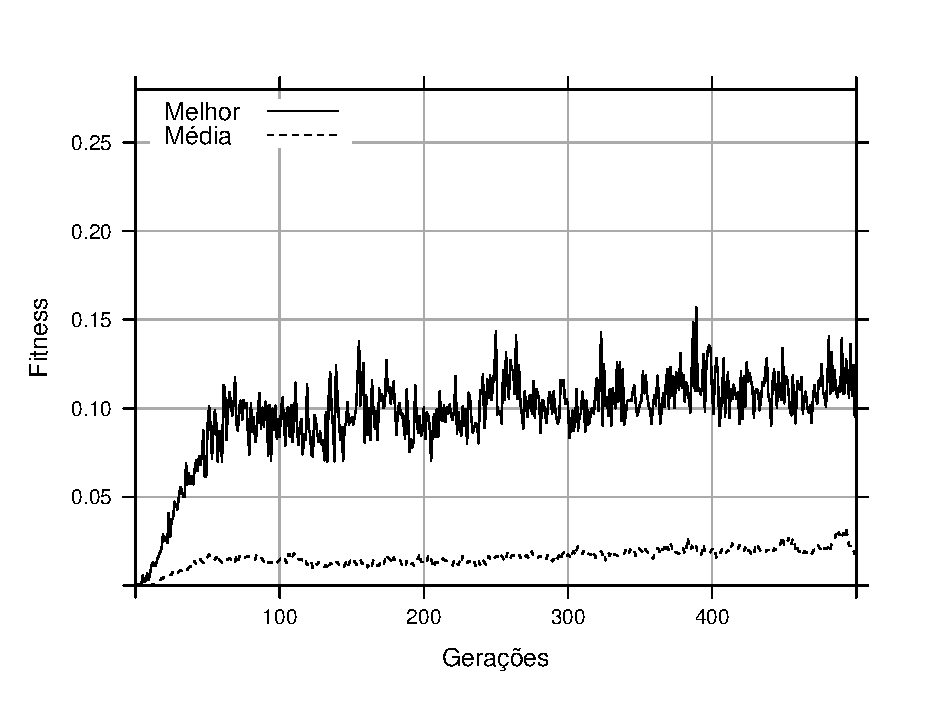
\includegraphics[width=\textwidth]{figures/fitness-f1}
        \subcaption{Função de \fitness \textbf{f1}}
    \end{minipage}%
    \begin{minipage}{.5\textwidth}
        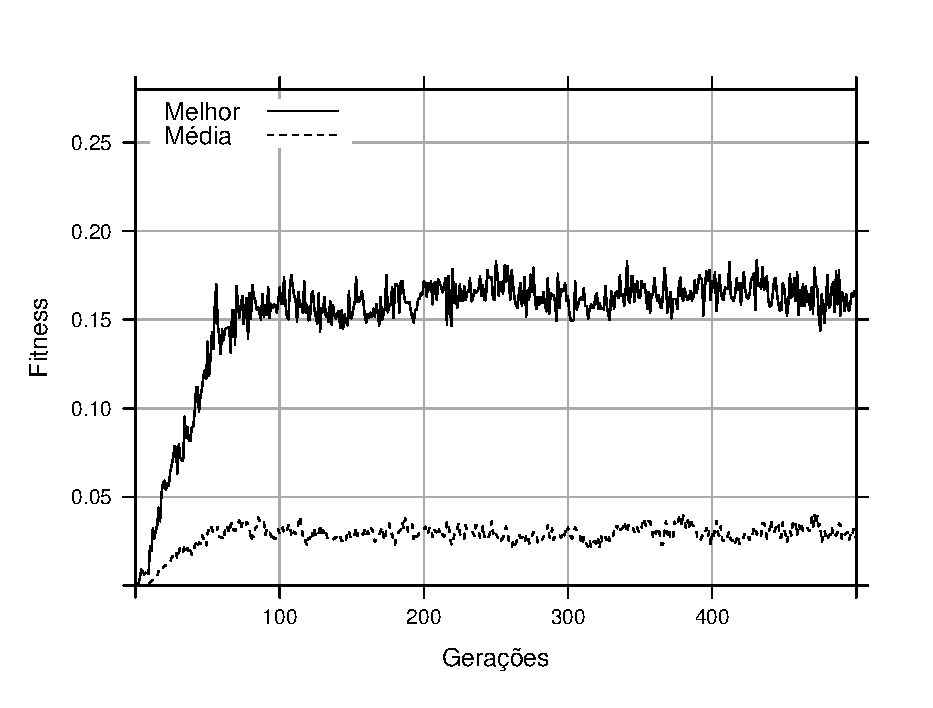
\includegraphics[width=\textwidth]{figures/fitness-f2}
        \subcaption{Função de \fitness \textbf{f2}}
    \end{minipage}

    \begin{minipage}{.5\textwidth}
        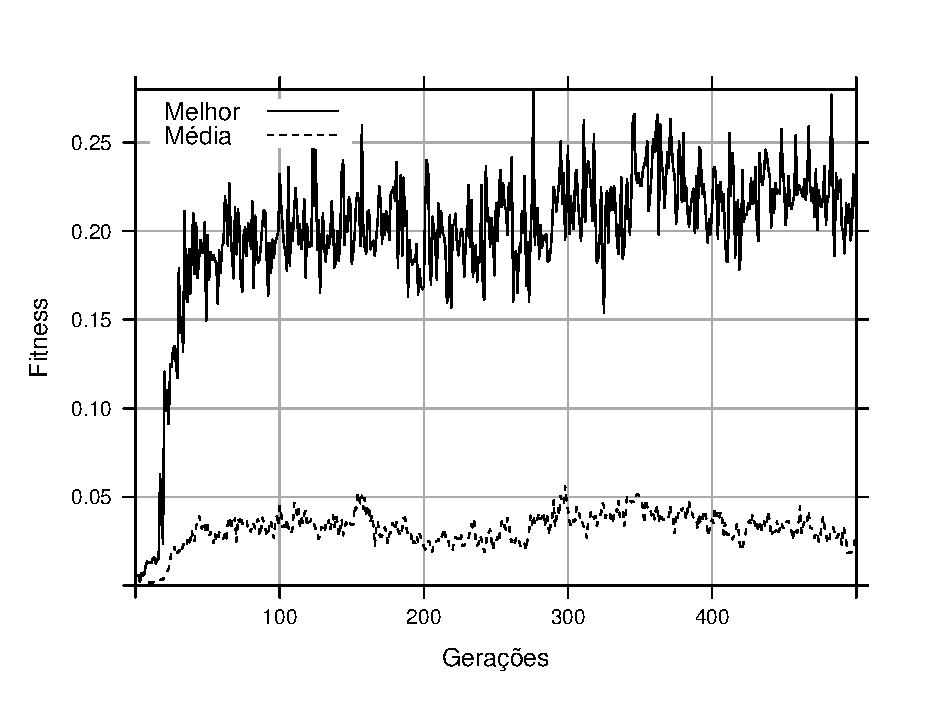
\includegraphics[width=\textwidth]{figures/fitness-f3}
        \subcaption{Função de \fitness \textbf{f3}}
    \end{minipage}%
    \begin{minipage}{.5\textwidth}
        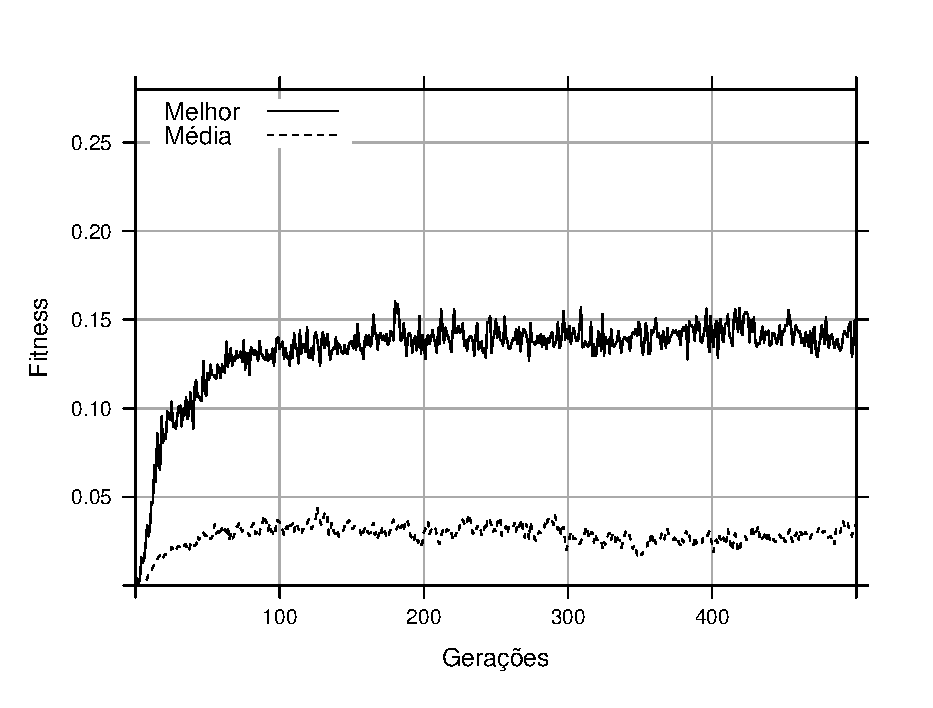
\includegraphics[width=\textwidth]{figures/fitness-f4}
        \subcaption{Função de \fitness \textbf{f4}}
    \end{minipage}

    \caption{Gráfico da \fitness do melhor indivíduo e média das \fitnessp dos indivíduos da população ao longo das gerações da execução de um GA para cada uma das quatro funções de \fitness.}
    \label{fig:func-fitness-gen}
\end{figure}

O melhor desempenho é apresentado pela função \textbf{f3} e o pior pela função \textbf{f1}.\\

A Figura \ref{fig:reeval} informa o resultado de 500 avaliações da função de \fitness simples (FFS -- que representa de forma mais fiel o ambiente real) a partir das soluções resultantes da execução de um GA para cada função de \fitness (ambientes de treinamento).

Contraditoriamente, o desempenho da função \textbf{f3} é o pior dentre os quatro nessas condições.

\begin{figure}[h]
    \centering
    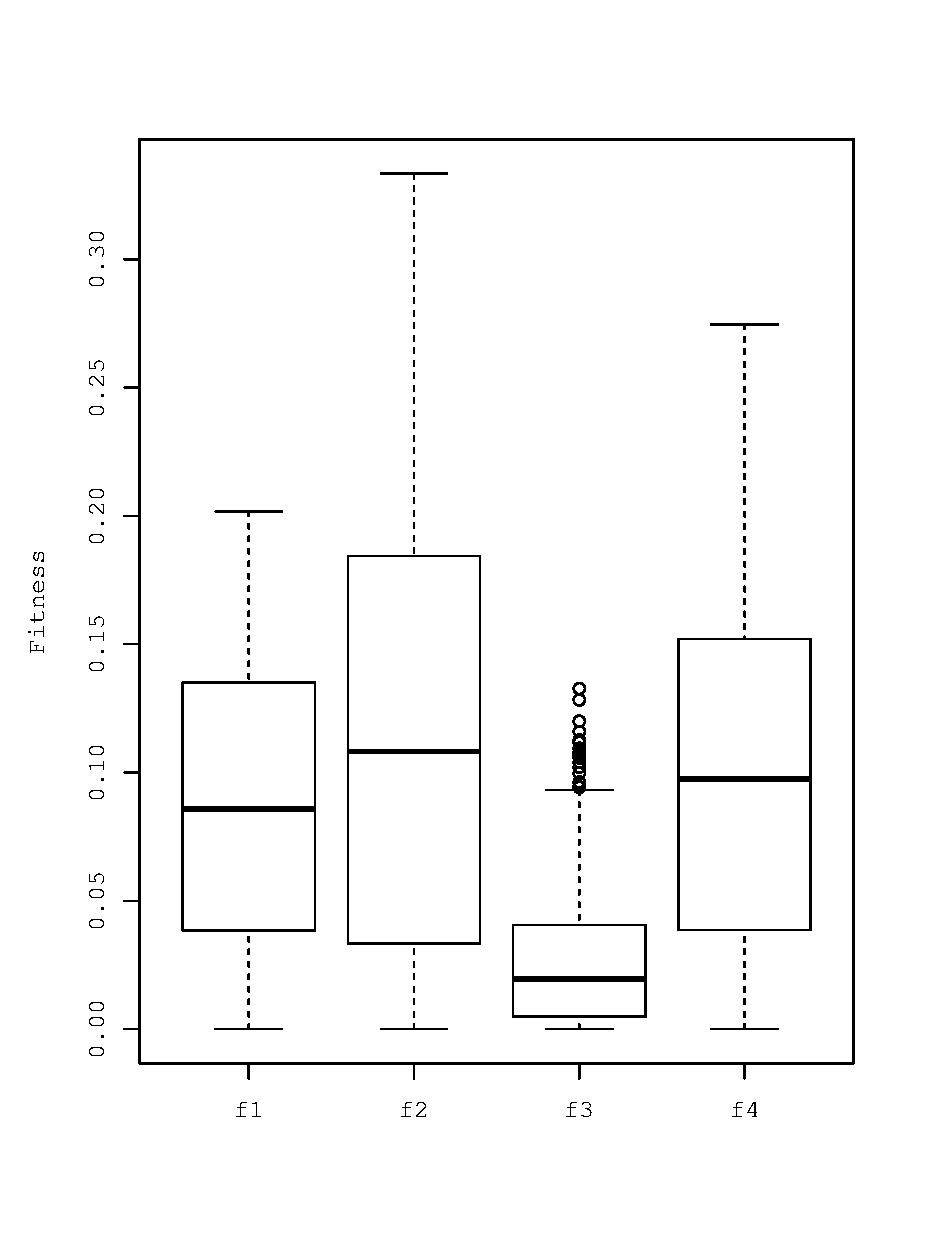
\includegraphics[width=.4\textwidth]{figures/reeval}
    \caption{Reavaliações}
    \label{fig:reeval}
\end{figure}

A solução resultante da execução com a função \textbf{f3} explora o fato de que a distância entre as áreas alvo é sempre a mesma para todos os testes, daí o baixo desempenho quando reavaliada no contexto da função objetivo (FFS) na qual a distância varia aleatoriamente.

As funções \textbf{f2} e \textbf{f4} de fato levam a melhores soluções do que a função \textbf{f1}. Como discutido na Seção \ref{sec:exp-fitness}, a aleatoriedade, mais presente na função \textbf{f1}, atrapalha a evolução.

Conclui-se que a redução de dificuldade da função de \fitness para que essa aproxime-se de uma função determinística pode levar a melhores soluções em problemas com muitas variáveis aleatórias. No entanto, essa redução pode expor alguma característica que pode ser explorada na fase de treinamento e, por consequência resultar em baixo desempenho da solução no ambiente real onde essa característica não é presente.

%%%%%%%%%%%%%%%%%%%%%%%%%%%%%%%%%%%%%%%%%%%%%%%%%%%%%%%%%%%%%%%%%%%%%%%%%%%%%%%%%%%%%%%%%%%%%%%%%%%

\section{Comparações entre algoritmos evolutivos}

A Figura \ref{fig:fitness-gen} apresenta a evolução das população ao longo das gerações para os quatro algoritmos evolutivos selecionados.

\begin{figure}[h]
    \centering
    \begin{minipage}{.5\textwidth}
        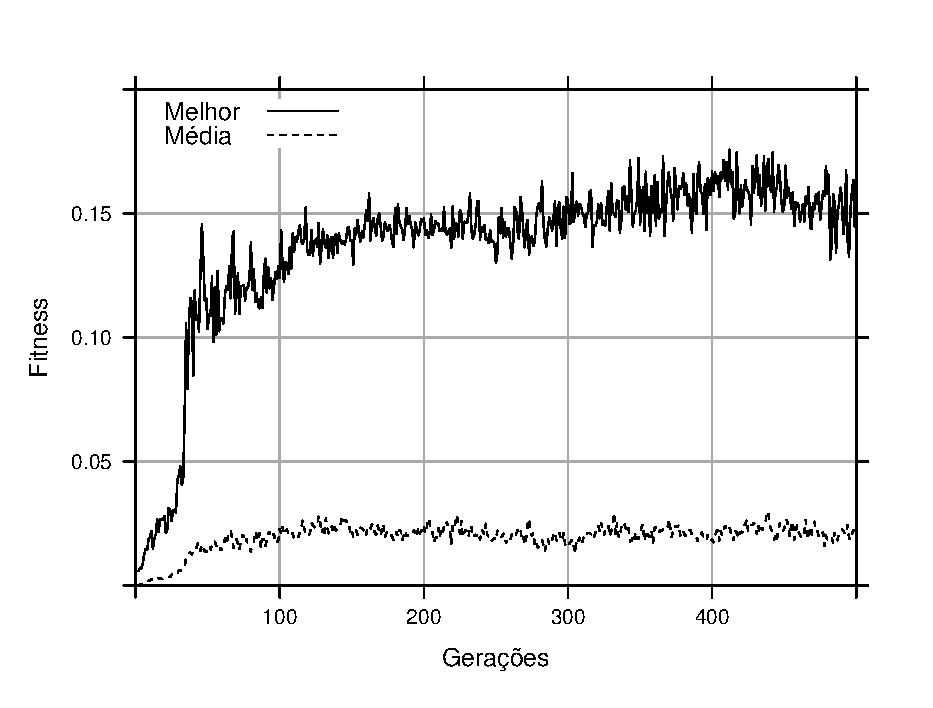
\includegraphics[width=\textwidth]{figures/fitness-GA}
        \subcaption{Execução de um GA}
    \end{minipage}%
    \begin{minipage}{.5\textwidth}
        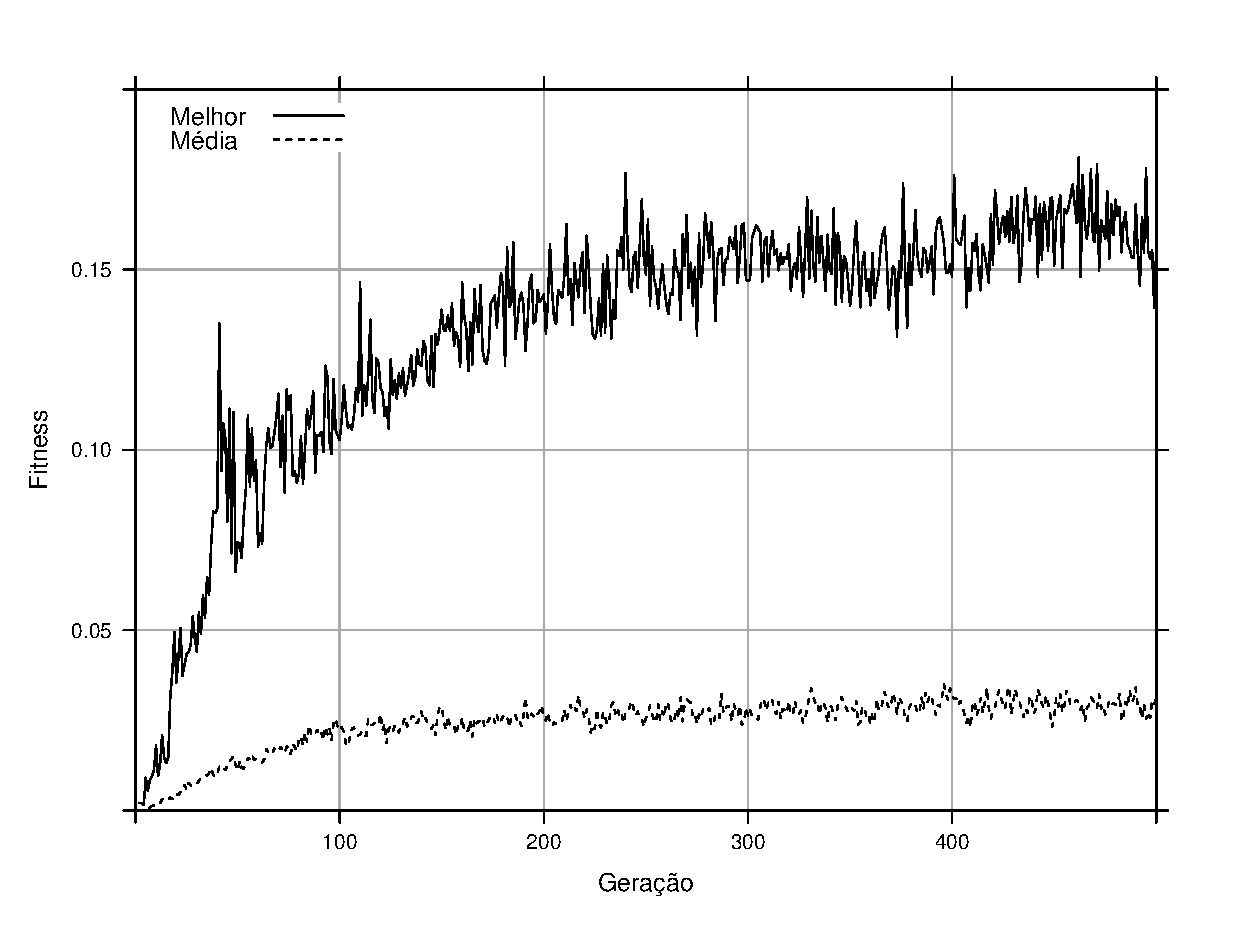
\includegraphics[width=\textwidth]{figures/fitness-PGA}
        \subcaption{Execução de um CGPGA}
    \end{minipage}

    \begin{minipage}{.5\textwidth}
        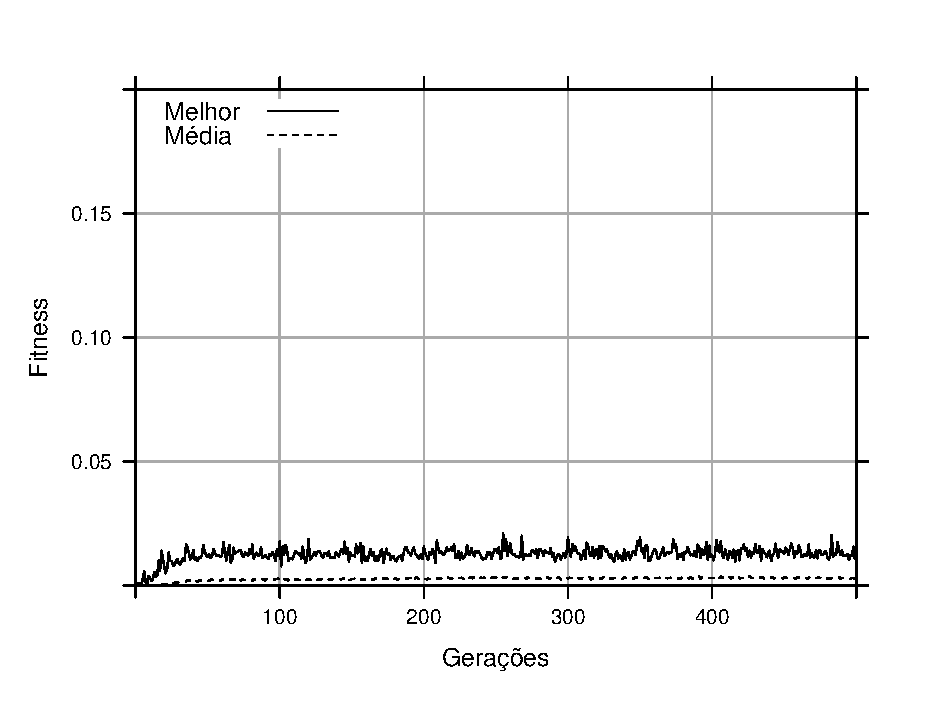
\includegraphics[width=\textwidth]{figures/fitness-PSO}
        \subcaption{Execução de um PSO}
    \end{minipage}%
    \begin{minipage}{.5\textwidth}
        \includegraphics[width=\textwidth]{figures/fitness-DPSO}
        \subcaption{Execução de um DPSO}
    \end{minipage}

    \caption{Gráfico da \fitness do melhor indivíduo e média das \fitnessp dos indivíduos da população ao longo das gerações de uma execução típica para cada um dos quatro algoritmos.}
    \label{fig:fitness-gen}
\end{figure}

